\section{LHCb Upgrade}\label{sec:LHCb_upgrade}
\subsection{Introduction}

The LHCb experiment is designed to detect the decay of long-lived particles, namely beauty and charmed mesons. As such, it is naturally suited for the search of BSM long-lived particles in a mass and lifetime range comparable to these mesons. It is the only LHC experiment to be fully instrumented in the forward region $2<\eta<5$, where $B$- and $D$-meson decays are abundant and their decay length is enhanced due to the large longitudinal boost. In this region, detector occupancy is extremely
high and the experiment has been run at reduced luminosity compared to ATLAS and CMS during Runs 1 and 2. However, an upgrade of the detector is planned to allow running at a luminosity of $2\times 10^{33}\,\,\text{cm}^{-2}\text{s}^{-1}$ in LHC Run 3 (starting in 2020) while maintaining or improving the current physics performance~\cite{LHCbUpgradeTDR}; this is 5 times larger than the luminosity during Runs 1 and 2. This first upgrade phase (Phase Ia) will entail a novel trigger paradigm where
all sub-detectors are fast enough to be read out in real time and the first trigger decisions are done in software. This trigger scheme is  extremely flexible and offers a great opportunity for searches of striking signatures like those of BSM long-lived particles. This upgrade comes earlier than the planned ATLAS and CMS upgrades for the HL-LHC phase which are planned to be installed during LHC long shutdown 3 (by 2025). In this shutdown, LHCb plans to consolidate and modestly enhance
the Phase-Ia upgrade detector (Phase Ib), while a Phase-II upgrade to run at an even higher luminosity up to $\sim 2\times 10^{34}\text{cm}^{-2}\,\,\text{s}^{-1}$ is planned to be installed later, during long shutdown 4 (by 2030)~\cite{LHCbUpgradeIIPC}. 

Section~\ref{sec:ulhcbperf} gives a brief overview of the Phase I upgraded-LHCb detector design and the expected performance of the LHCb sub-detectors. 
An overview of the upgraded LHCb capabilities in the context of LLP searches is given in Section~\ref{sec:ulhcbphys} with a few example signatures. 
Finally, an overview of the plans for the Phase-II upgrade and some thoughts on the opportunities given by putative additional detector features are reported in Section~\ref{sec:ulhcbphaseii}.



\subsection{LHCb detector and trigger upgrade for Run 3 (Phase Ia)}
\label{sec:ulhcbperf}

In LHC Run 3, LHCb plans to take data at an instantaneous luminosity of $2\times 10^{33}\,\,\text{cm}^{-2}\text{s}^{-1}$, a factor of five larger than the current luminosity. The LHCb detector needs to be upgraded to cope with the higher radiation dose and, most importantly, to avoid the saturation of the trigger rate and exploit the higher luminosity. The main bottleneck in the current trigger is in the first stage, which reduces the accepted rate from 30 MHz to 1 MHz  at hardware level. For the upgrade, the hardware trigger will be removed and the full event will be read out at the bunch crossing rate of the LHC (40~MHz), with a very flexible software-based trigger. \\

\begin{table}[h!]
    \centering
    \begin{tabular}{lrrrr}
         & Current & Phase-Ia & Phase-Ib & Phase-II \\
        \hline
      ${\cal L} / (\text{cm}^{-2}\text{s}^{-1})$ & $4 \times 10^{32}$ & $2 \times 10^{33}$ & $2 \times 10^{33}$ & $2 \times 10^{34}$\\
        $\int_{ } \cal L$   & 8\invfb & 23\invfb & 50\invfb & 300\invfb \\
        $\sqrt{\text{s}}$       & 7, 8, 13~TeV & 14 TeV & 14 TeV & 14 TeV \\
        $\mu$    & $\sim 1$ & $\sim 5$ & $\sim 5$ & $\sim 50$ \\
        \hline
    \end{tabular}
    \caption{LHCb current and upgraded operating conditions~\cite{LHCbUpgradeIIPC}. Instantaneous luminosity $\cal L$, integrated luminosity $\int_{ } \cal L$ (including previous runs), $pp$ collision energy $\sqrt{s}$ and average number of visible proton interactions $\mu$ are listed.}
    \label{tab:cond}
\end{table}

Table \ref{tab:cond} summarises the current and upgraded conditions of the detector. To cope with the larger occupancy and higher rate of the upgraded detector, the electronics of all of the sub-detectors must be upgraded, and some sub-detectors must be fully replaced; for example, the tracking system, which plays a crucial role in LLP searches, must be replaced.\\

The upgraded tracking system consists of the VErtex LOcator (VELO), surrounding the interaction point, the Upstream Tracker (UT), a tracking station placed before the magnet, and the Scintillating Fibers tracker (SciFi), three stations after the magnet. 
In the VELO~\cite{LHCb-TDR-013}, the current strips will be replaced by pixel detectors, with a custom developed ASIC (VeloPix) able to withstand a maximum hit rate of 900 Mhits/s/ASIC. The UT~\cite{LHCb-TDR-015} is composed of four silicon micro-strip planes, with finer granularity and larger acceptance compared to the current tracker. Each station of the SciFi has four planes of 2.5 m long scintillating fibres read out by silicon photo-multipliers.

The upgrade components most important for LLP searches are probably the  VELO, the tracking and the software trigger. In the following subsections a brief description of their design and capabilities is given for each.


\subsubsection{VELO Upgrade}
The VELO plays a fundamental role in LLP searches at LHCb:~due to the large boost particles typically get in the forward direction, a very precise measurement of the LLP vertex position allows LHCb to access very low lifetimes that are often not accessible at ATLAS and CMS.

In upgrade conditions, the number of tracks and primary vertices will increase by about a factor of five, making it much more difficult to identify displaced vertices close to the beam-line; it is an additional challenge to do this in real time.
The VELO was thus completely redesigned~\cite{LHCb-TDR-013} to cope with the new high-luminosity conditions, maintaining high physics performance and allowing real-time readout for the software trigger. The new VELO has a pixel rather than strip geometry and its distance from the LHC beams is reduced from 8 to 5~mm. This allows  an improvement in the vertex resolution (see Fig.~\ref{fig:ulhcb_pvres}) and reduces the rate of unphysical (ghost) tracks.

\begin{figure}[t]
\centerline{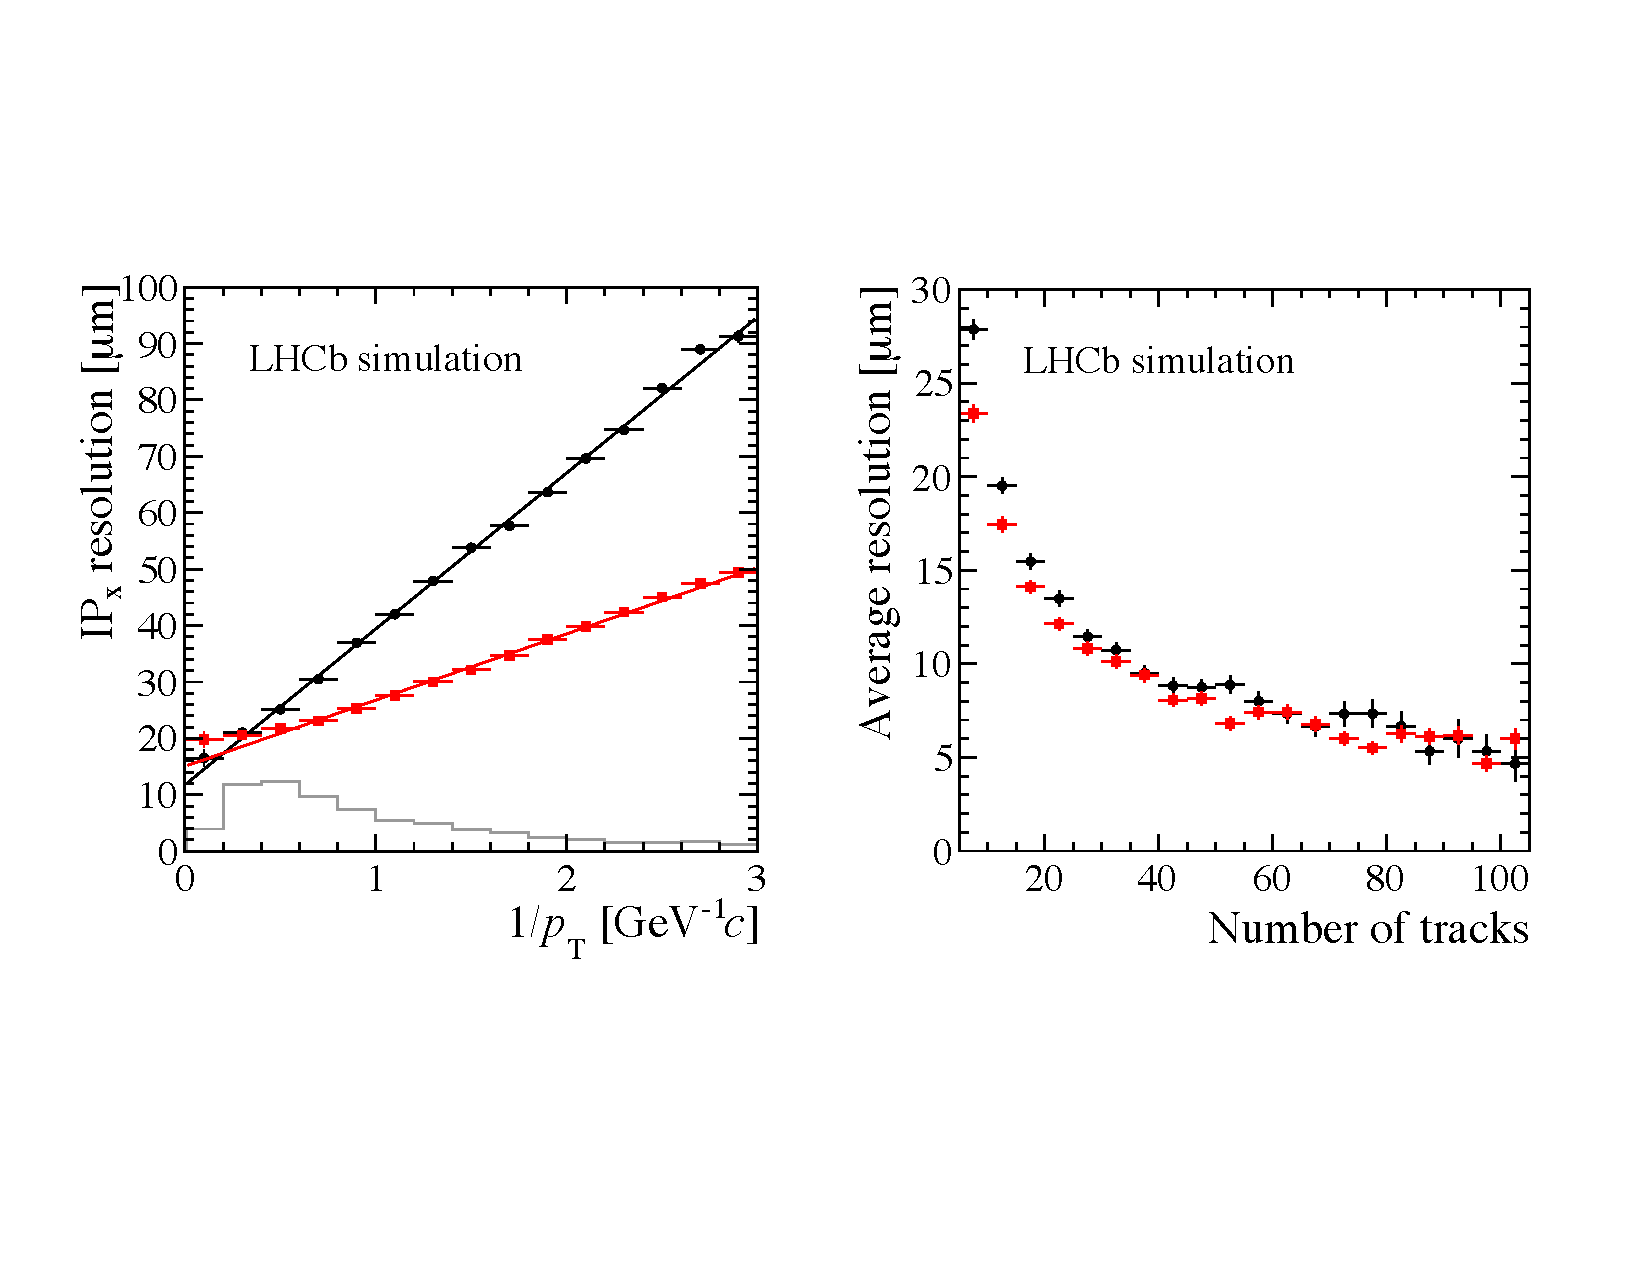
\includegraphics[width=\textwidth]{figures/lhcb_vertexres.pdf}}
  \caption{Resolution of the primary vertex as a function of number of tracks in the $x$ (left) and $z$ (right) direction. The same kind of improvement is also expected for secondary vertices (SV).}
  \label{fig:ulhcb_pvres}
\end{figure}

The pattern recognition efficiency for track reconstruction is superior to the one of the current VELO when evaluated in high-luminosity conditions. Particularly important for LLP searches is the efficiency of track reconstruction as a function of the displacement from the origin along the beam axis:~for the upgraded VELO, the efficiency approaches $100\%$ and is uniform in a window of 20 cm around the interaction point, thanks to the new configuration of the modules in the $z$ direction and the shorter distance from the beam. The VELO acceptance degrades quickly after 20 cm in $z$, giving an upper limit for LLP decay lengths with vertices reconstructible in the VELO. A display of the upgraded VELO geometry and its acceptance in both the forward and backward directions is given in Figure~\ref{fig:ulhcb_veloacc}.

Another important metric of   detector performance  is the impact parameter  resolution, especially in LLP searches where it can be exploited to reduce the background due to fake tracks. With the upgrade, the impact parameter resolution  significantly improves for low \pt tracks. For example, the impact parameter resolution along $x$ for tracks with \pt of 0.5\gev is $40\,\,\mu{\rm m}$ in the upgrade versus $70\,\,\mu\mathrm{m}$ in the current VELO. 
The replacement of strips with pixel sensors also makes the pattern recognition faster for the same multiplicity. This can be used in the trigger to find tracks and identify displaced vertices in the trigger, making it possible to soften or remove inefficient $\pt$ requirements.

\begin{figure}[t]
  \centerline{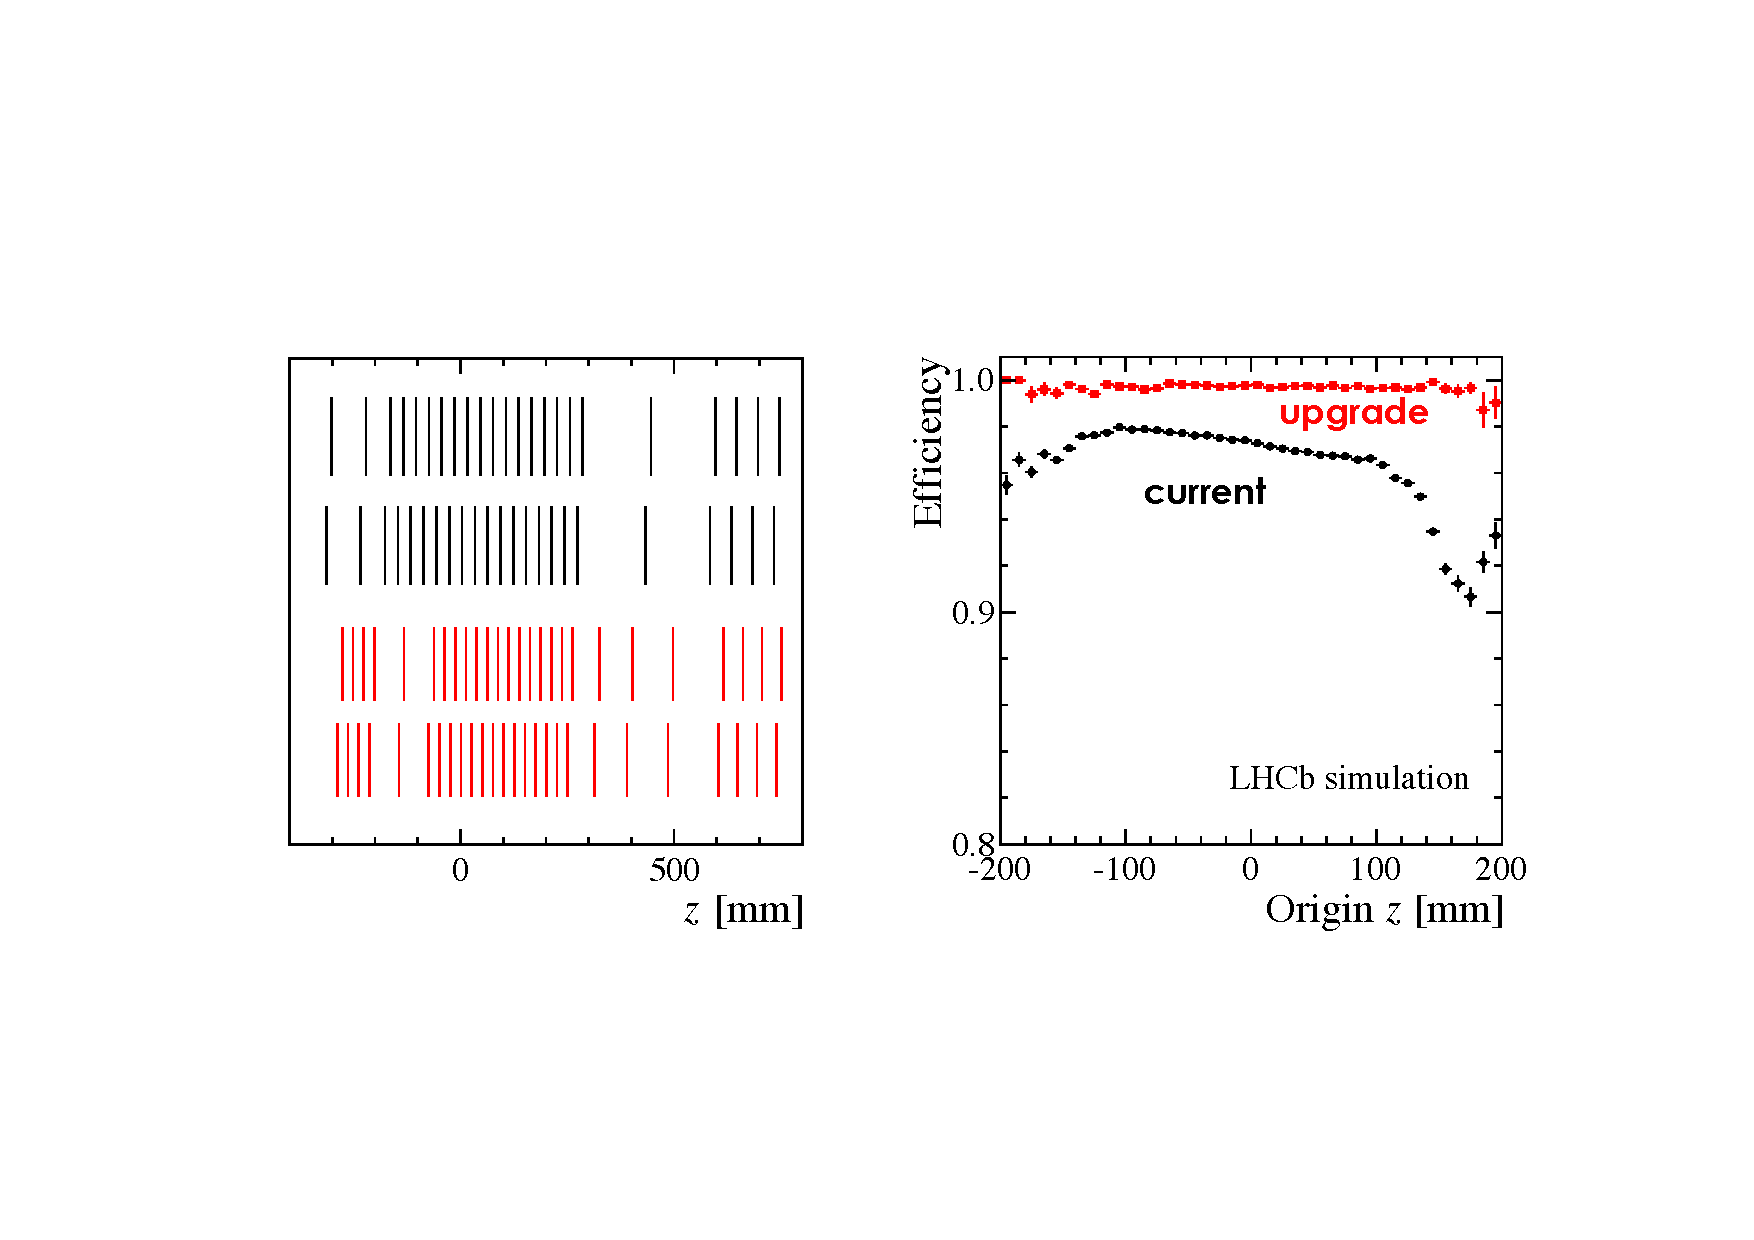
\includegraphics[width=\textwidth]{figures/lhcb_veloperf.pdf}}
  \caption{A comparison of the current and upgrade VELO $z-$layouts is shown on the left. The top layout (black) is the current VELO while the bottom layout (red) is the upgrade VELO. On the right the track reconstruction efficiency is shown as a function of the origin in $z$ for the current (black) and upgrade (black) VELO in upgrade conditions.}
  \label{fig:eff}
\end{figure}

\begin{figure}[h]
\centerline{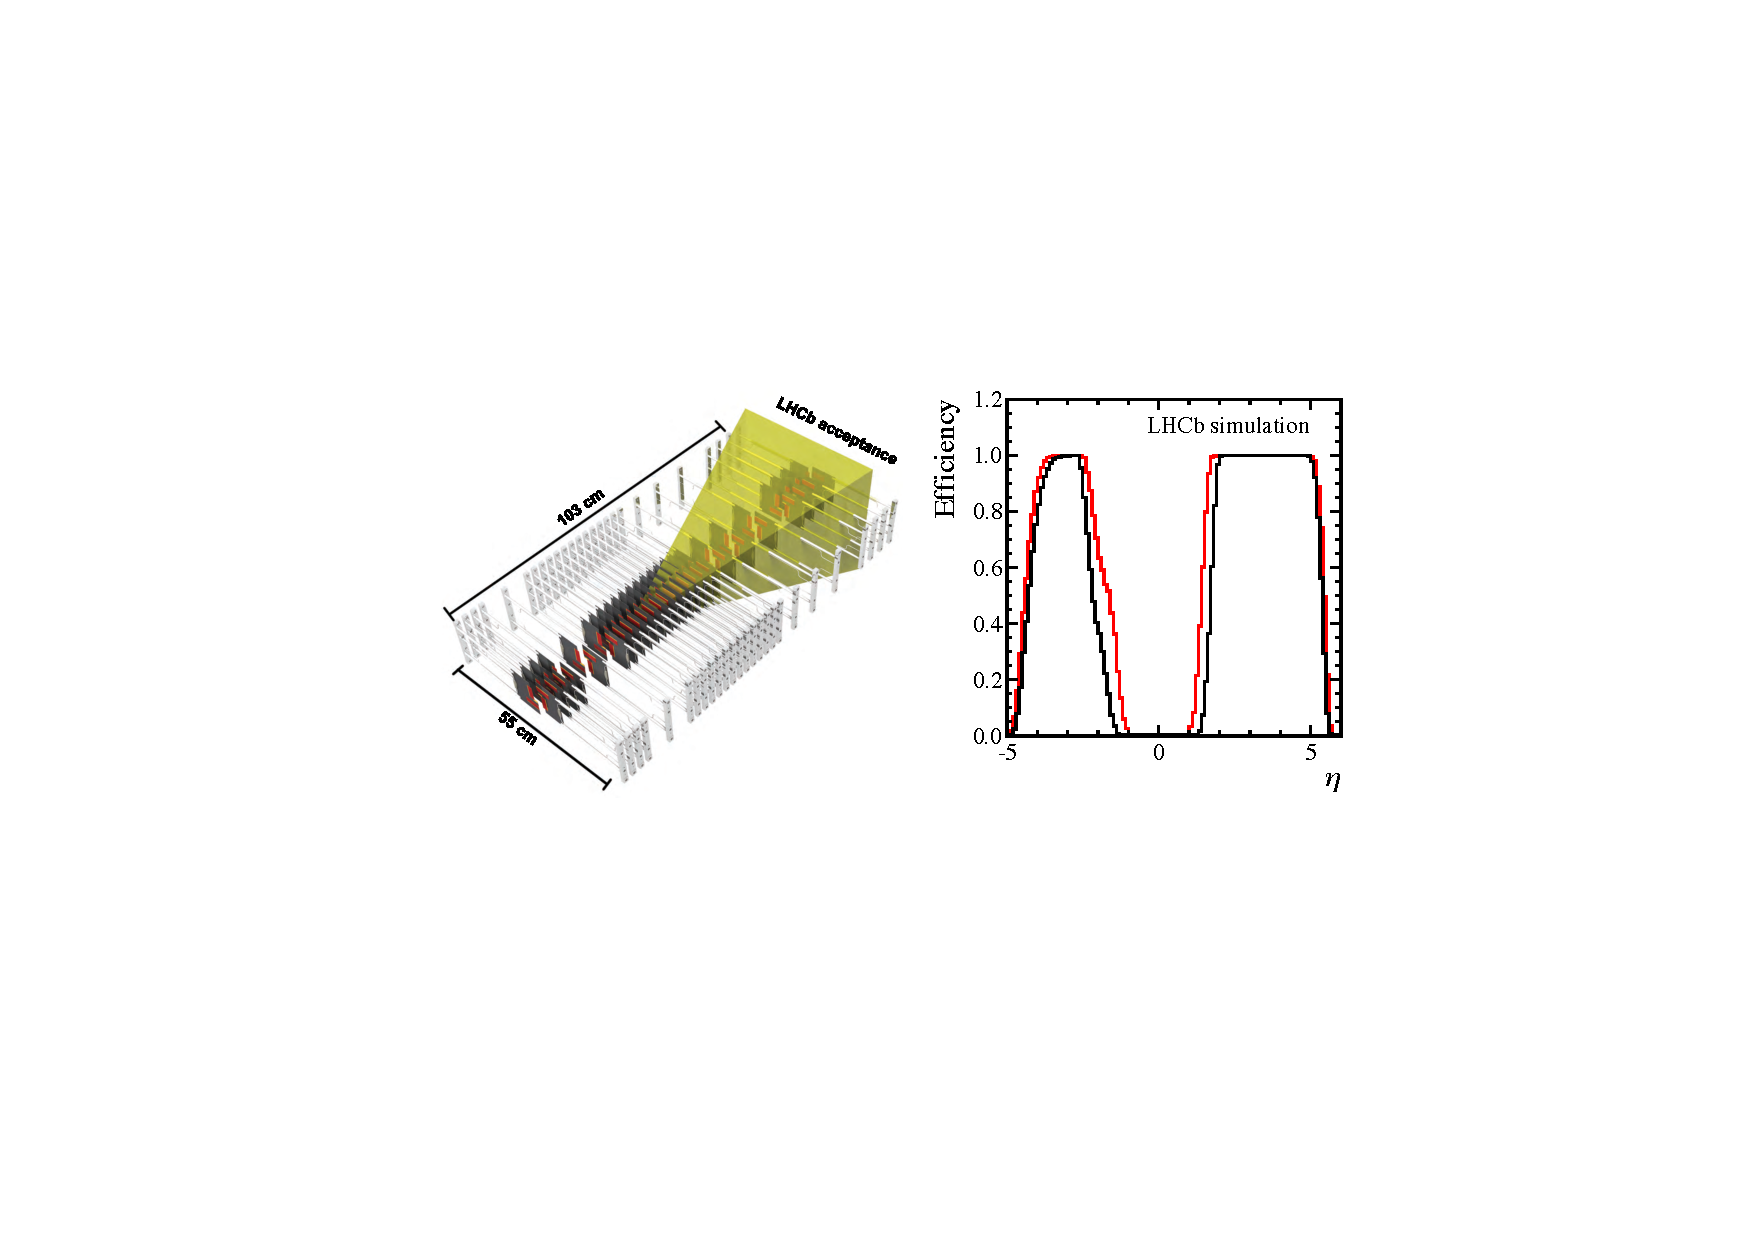
\includegraphics[width=\textwidth]{figures/lhcb_veloacceptance2.pdf}}
  \caption{On the left is a display of the upgrade VELO geometry and a comparison with the LHCb spectrometer acceptance which is shaded in yellow. On the right the $\eta$ acceptance of the upgrade VELO geometry is given both for forward and backward tracks. The fraction of tracks crossing three and four modules is given in red and black, respectively.}
  \label{fig:ulhcb_veloacc}
\end{figure}

Real displaced tracks created by interactions in the VELO material can be a significant background to LLP searches (see more details in Chapter~\ref{sec:backgrounds}). The total material budget of the upgraded VELO is similar to the current detector (with a radiation length of about $20\%$) and is dominated by interactions in the Radio-Frequency foil separating the beam vacuum from the vacuum of the sensors.
However, the average percentage of radiation length before the first measured point is significantly reduced in the upgrade VELO, passing from $4.6\%X_0$ in the current design to $1.7\%X_0$ in the upgraded VELO (where $X_0$ is the radiation length).

\subsubsection{Upgraded trigger}

The online event selection in the LHCb experiment during the 2010-2018 running period is performed by a trigger composed of a hardware level (L0), and two software levels:~High Level Trigger 1 (HLT1) and High Level Trigger 2 (HLT2). The L0 reduces the rate from 40 MHz (the LHC bunch-crossing rate) to 1 MHz using information from the calorimeter and muon systems. Typical requirements in the L0 are $\pt>1.4\gev$ for muons and $E>2.5\gev$ for electrons. The software trigger performs a partial
event reconstruction at HLT1, reconstructing tracks and primary vertices for any particle down to $\pt=500\mev$, followed by a complete event reconstruction at HLT2, reducing further the rate to 12.5 kHz (in LHC Run 2).

In the Phase-I upgrade, LHCb foresees to run at a luminosity of $2\times 10^{33}\,\,{\rm cm}^{-2}{\rm s}^{-1}$, about a factor of 5 larger than the one that it run at during LHC Run 2.
For this reason, a new trigger system, able to fully exploit the LHC potential, has been designed~\cite{LHCb-TDR-016, Aaij:2244312}.
The upgraded LHCb trigger consists of two paradigms, a triggerless readout and a full software trigger. 
In addition, as already tested in Run 2, a real-time alignment and calibration will achieve offline-quality reconstruction already in the trigger, allowing a higher signal purity of interesting decay channels. Figure~\ref{fig:ulhcb_trigger} shows the current and the upgraded trigger schemes. 

\begin{figure}[t]
\centerline{
 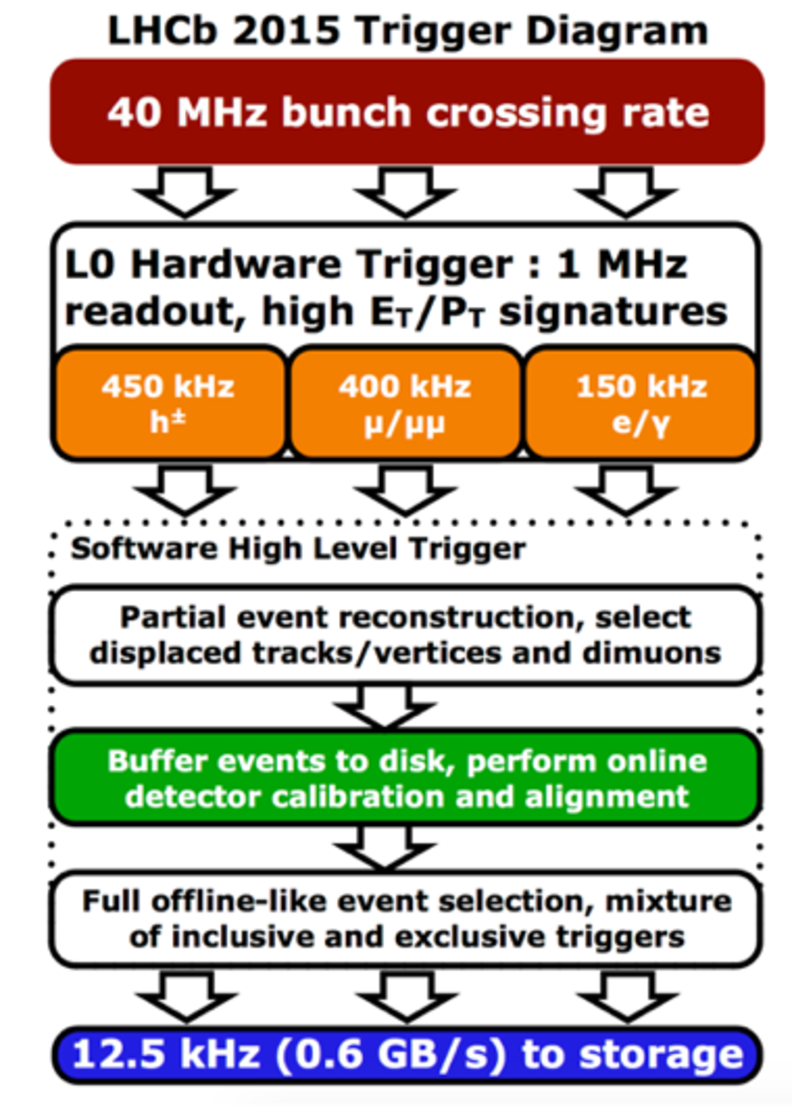
\includegraphics[width=0.5\textwidth]{figures/Trigger2015.pdf}\\
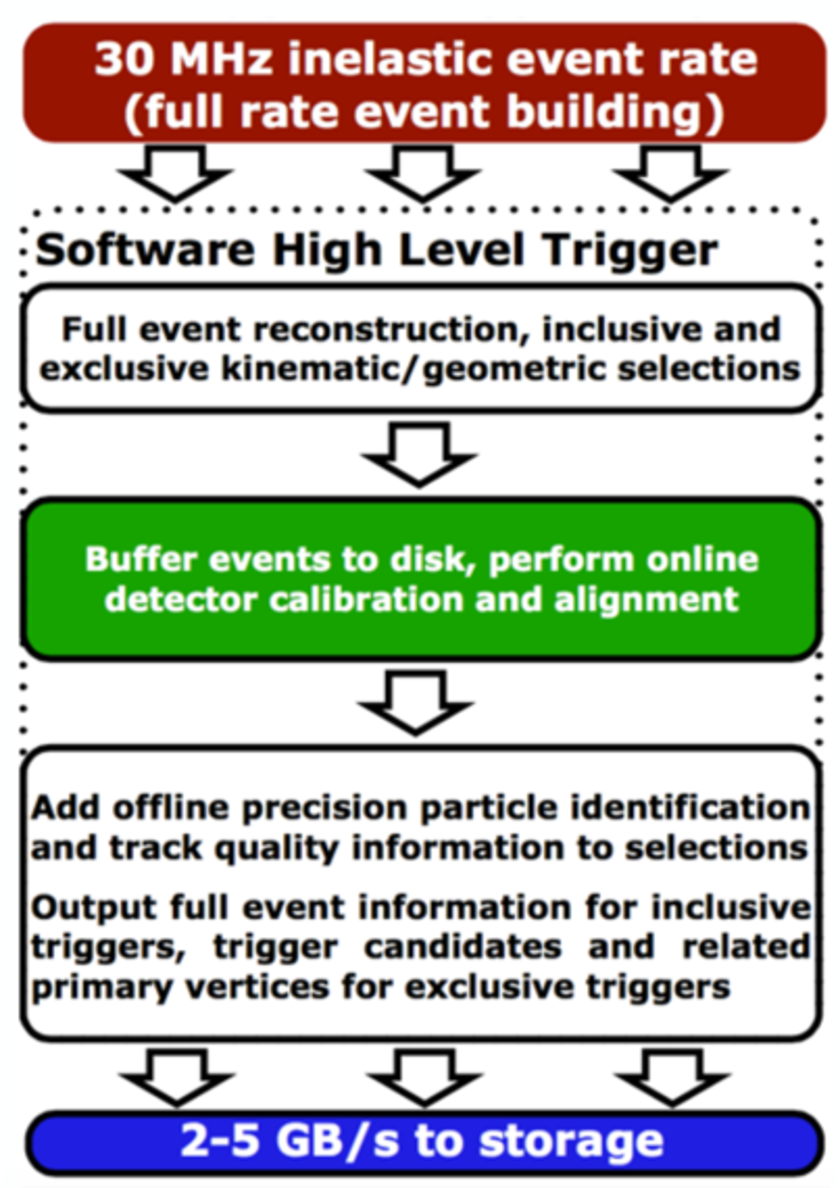
\includegraphics[width=0.5\textwidth]{figures/TriggerUpgrade.pdf}	}
  \caption{Scheme of the current trigger (left); and of the upgraded LHCb trigger (right).}
  \label{fig:ulhcb_trigger}
\end{figure}

\paragraph{Triggerless readout and full-software trigger}
With the LHCb trigger upgrade, the 1 MHz readout limitation will be removed, allowing the full event rate to be processed in software. This will increase the efficiency for several channels which otherwise would not benefit from the higher luminosity because they would saturate the L0 trigger rate. Figure~\ref{fig:triggervsLumi} shows how the rate for non-muonic $B$ decays saturates the L0 trigger with increasing luminosity. Most of these channels saturate the L0 trigger already at the Run-2 luminosity ($4\times
10^{32}\,\,{\rm cm}^{-2}{\rm s}^{-1}$).
Moreover, a purely software trigger will not require the $\pt$ requirements currently applied at the hardware trigger level. Several physics program involving low-$\pt$ particle, currently prevented because of the low L0 efficiency, will therefore become possible.

\begin{figure}[t]
\centerline{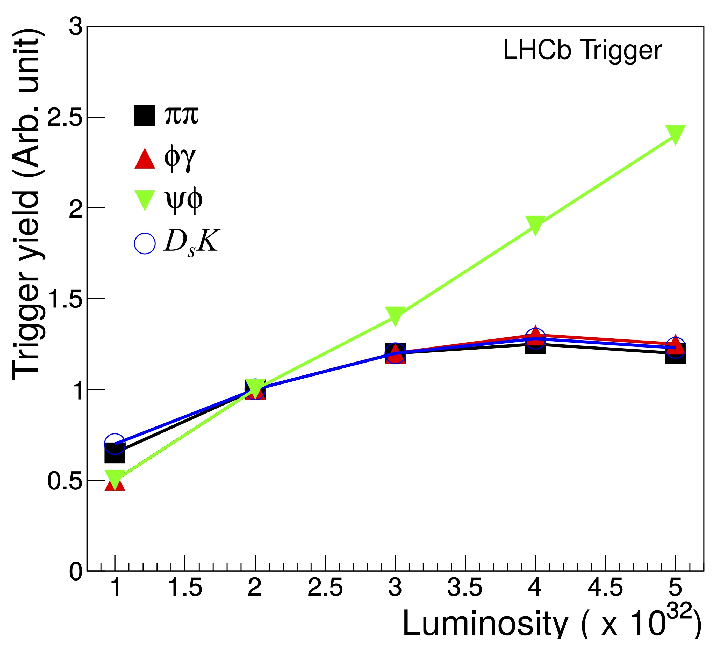
\includegraphics[width=0.6\textwidth]{figures/L0vsLumi.pdf}}
\caption{Trigger yields for ${B\to\pi^+\pi^-}$, ${B_s\to\phi(K^+K^-)\gamma}$, ${B_s\to J/\psi(\mu^+\mu^-)\phi(K^+K^-)}$ and ${B_s\to D_s^-(K^+K^-\pi^-)K^+}$ as a function of the luminosity with the current trigger. For non-muonic channels, the saturation effect due to the L0 trigger can be observed.}
  \label{fig:triggervsLumi}
\end{figure}

\paragraph{Turbo Stream}
Starting from Run 2, offline-quality alignment and calibration is applied between the HLT1 and the HLT2 levels. This made possible the design of a new dedicated
trigger output called Turbo Stream. The event record is written directly from the trigger and processed by the Tesla application~\cite{Aaij:2016rxn}, and its output can be directly used for physics analysis without the need for offline reconstruction.
Several variations of Turbo have been introduced in the last several years. For the 2015 data taking, the first version of Turbo allowed only the exclusive triggered candidate to be saved, without keeping the rest of the event and discarding all sub-detector information. 
While the event size was an order of magnitude smaller than for full stream data, any analysis relying on additional information from the surrounding event could not use Turbo Stream data. 
For this reason, full event reconstruction was implemented as Turbo++ in 2016. Finally, a new intermediate solution between Turbo and Turbo++ called Turbo SP (Selective Persistence) was implemented in 2017. With Turbo SP, both the trigger candidate and a subset of the reconstructed event are saved. This extremely flexible solution allows the analyzer to choose which objects to save, minimizing the size of the stored event. A sketch of the evolution of Turbo is shown in Figure~\ref{fig:turbo}.
Once the trigger is upgraded to run purely at the software level, Turbo becomes the only available solution. The reduced event size allows the storage of particle candidates at a high rate, fully exploiting the reduction in \pt thresholds due to the removal of the L0 hardware trigger.  

\begin{figure}[t]
\centerline{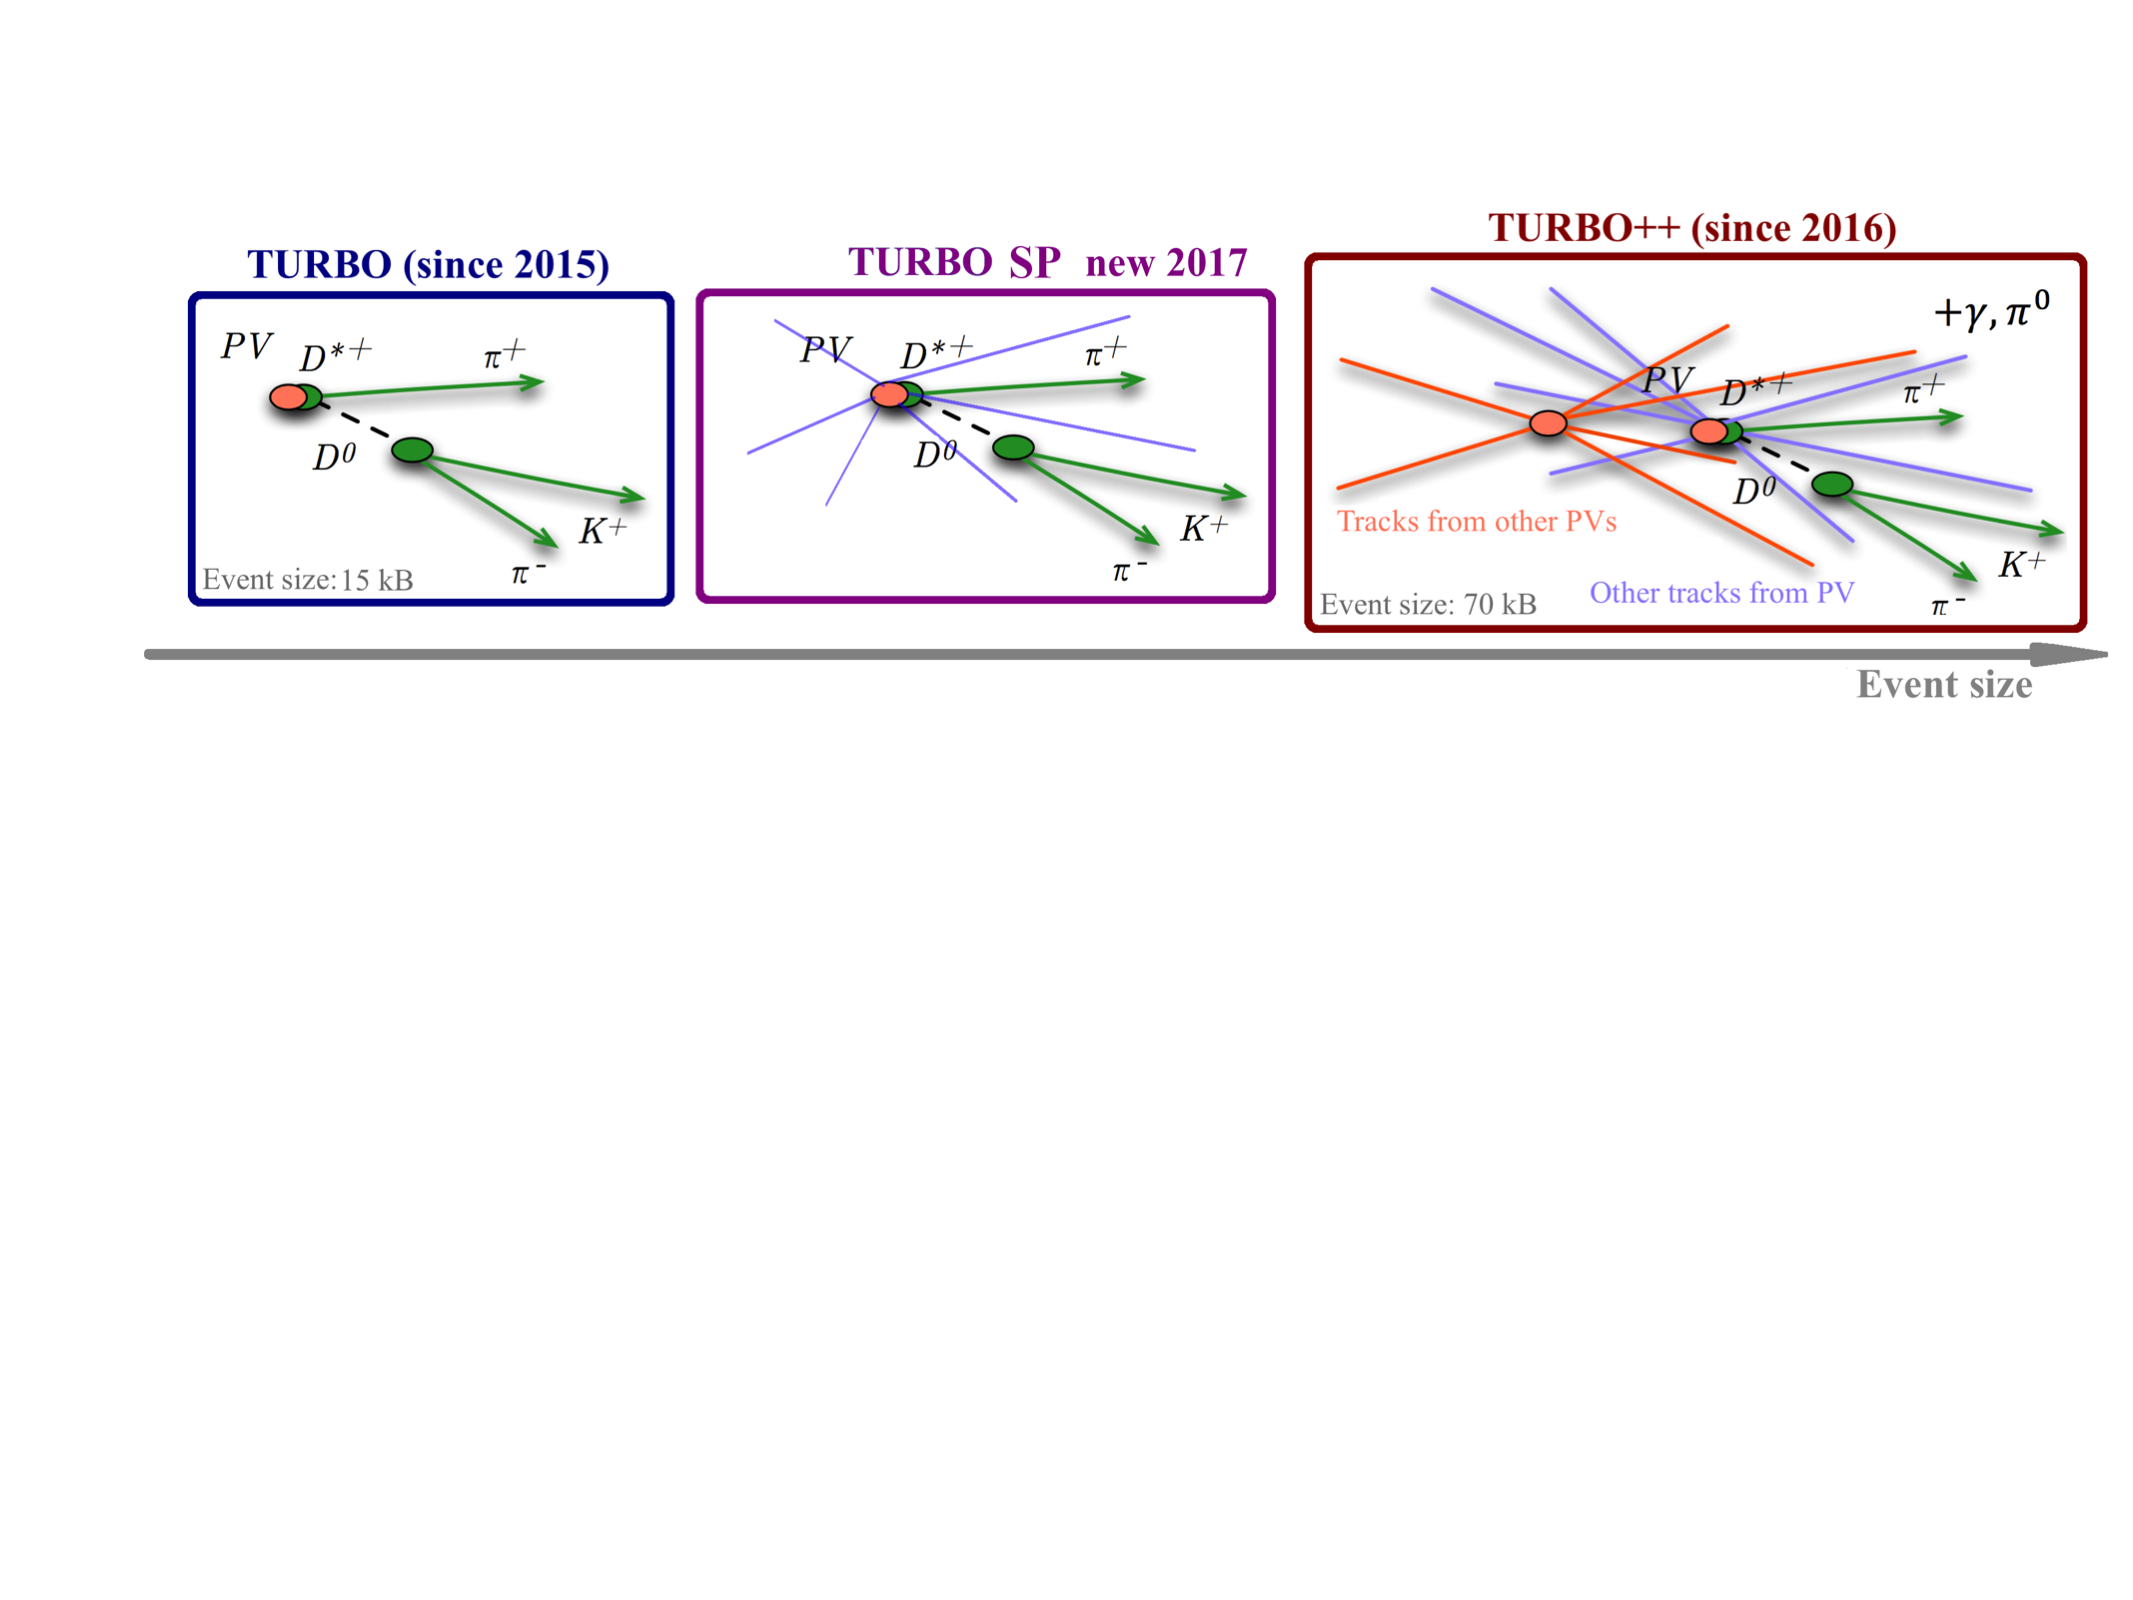
\includegraphics[width=1.05\textwidth]{figures/Turbo.pdf}}
  \caption{Sketch of the evolution of Turbo.}
  \label{fig:turbo}
\end{figure}




\subsection{LHCb Upgrade Ia Projections for LLP Signatures}
\label{sec:ulhcbphys}

The much higher luminosity and improved capabilities of the upgraded LHCb detector are expected to significantkly improve the LHCb capabilities for LLP searches in LHC Run 3. In the following sections, the projected sensitivity to several benchmark LLP signatures are shown to showcase the potential of the upgraded detector. However, the potential of the upgraded triggerless readout has not been completely explored yet and its great flexibility could be exploited in several ways beyond those shown here.

\subsubsection{Displaced di-leptons}
The upgraded LHCb experiment is expected to have exceptional sensitivity to low-mass displaced dilepton signatures thanks to the mass resolution, excellent vertexing, and the online selection allowed by the triggerless readout.

The upgrade LHCb sensitivity to dileptons has been explored in the literature in the context of dark photon searches. Two complementary signatures have been considered:~an inclusive search for BSM gauge bosons (dark photons) in $A'\to \mu^+\mu^-$, and a search for  $A'$ using radiative charm decays $D^{*0}\to D^{0}A',\,A'\rightarrow e^+e^-$.
The inclusive search~\cite{Ilten:2016tkc} scans a very large region from the dimuon threshold $2m_{\mu}$ all the way up to the $Z$ pole. The second proposed signature~\cite{Ilten:2015hya} exploits a tag of the radiative decay of the $D^{*0}$ using its reconstructed invariant mass and a di-electron dark photon final state to probe a much lower mass range allowed by the decay kinematics, $[2m_{e}$,142 MeV$]$.
For both signatures, three non-overlapping search regions are defined according to different requirements on the $A'$ flight distance:
%
\begin{itemize}
\item prompt resonant;
\item displaced upstream of the first VELO module;
\item displaced downstream of the first VELO module.
\end{itemize}
%
The prompt search is expected to probe mixing parameters $\epsilon^2$ below $10^{-7}$ despite the large irreducible background from Drell-Yan and QCD\footnote{In the limit $m_{A'}\ll m_Z$, the coupling of the dark photon to SM particles with charge $Q$ is approximately $Qe\epsilon$.}.
Since the dark photons with masses above the $\eta$ mass decay promptly for couplings that are accessible within LHCb, no attempt is made to probe displaced dark photons in that region.

An inclusive search for dark photons has already been performed with Run 2 data~\cite{Aaij:2017rft}. This was possible due to the high reconstruction and identification efficiency of soft di-muons at LHCb. These results demonstrated the unique sensitivity that can be reached at LHCb. The planned increase in luminosity and removal of the hardware-trigger stage in Run 3 should increase the number of expected $A'\to \mu\mu$ decays in the low-mass region by a factor of ${\cal O}(100-1000)$ compared to the 2016 data sample. The limits placed by the current data and the sensitivity expected with future LHC runs is shown in Figure~\ref{fig:lhcb_darkph}.

The exclusive search for $D^{*0}\to D^{0}A',\,A'\rightarrow e^+e^-$ is much more challenging and not feasible prior to the upgrade, since the hardware trigger and the thicker RF foil degrade the sensitivity. This search highly relies on the online identification of $e^{+}e^{-}$ pairs, since over 5 trillions of these $D^{*0}$ decays are expected in Run 3. The expected sensitivity probes unexplored regions of phase space at very low $A'$ mass and mixing $\epsilon^2$ that is usually in the realm of beam-dump experiments.

\begin{figure}[t]
  \centerline{\includegraphics[width=\textwidth]{figures/lhcb_darkphoton_projections.pdf}}
  \caption{Current and expected limits in the dark photon parameter space mixing $\epsilon^2$ versus $A'$ mass~\cite{LHCbUpgradeIIPC}. The black line represents current LHCb limits from Ref.~\cite{Aaij:2017rft}, while grey-shaded regions are existing limits from other experiments. Expected limits from the proposed inclusive search with 50 and 500 \invfb are shown in shades of blue. The expected sensitivity of $D^{*0}\to D^{0}A'(ee)$ at low mass is shown in shades of green. The arrows indicate the available
mass range from light meson decays into $e^+e^-\gamma$.}
  \label{fig:lhcb_darkph}
\end{figure}

A displaced di-muon signature also appears in some Hidden-Valley (HV) scenarios \cite{Strassler:2006im}, in which a hidden sector with strong dynamics showers and hadronizes into  dark mesons that can have an appreciable decay rate to leptons. For more information on dark showers, see Chapter \ref{sec:showers}. The upgraded LHCb prospects for this type of signature have been explored in Ref.~\cite{Pierce:2017taw} and are extremely promising.
In the scenario explored in Ref.~\cite{Pierce:2017taw}, dark mesons are produced with large multiplicities between 10 and 30. Selection criteria inspired by the proposed dark photon search~\cite{Ilten:2016tkc} in the region after the first VELO module are applied.
The expected reach for the proposed searches using Run 3 data from LHCb (15 \invfb) and from ATLAS/CMS (300 \invfb) are shown in Fig.~\ref{fig:ulhcb_hv_dimuons}. The model studied involves a 200 \gev $U(1)'$ gauge boson $Z_p$ decaying to a HV quark pair; showering and hadronization in the dark sector leads to a large multiplicity of hidden hadrons $\omega_V$ (with $m_{\omega_V} =0.3\,\,\gevcc$) that can decay to di-muons. In this context, the upgraded LHCb detector could have better sensitivity than other proposed searches at ATLAS and CMS. 

\begin{figure}[t]
  \centering
  {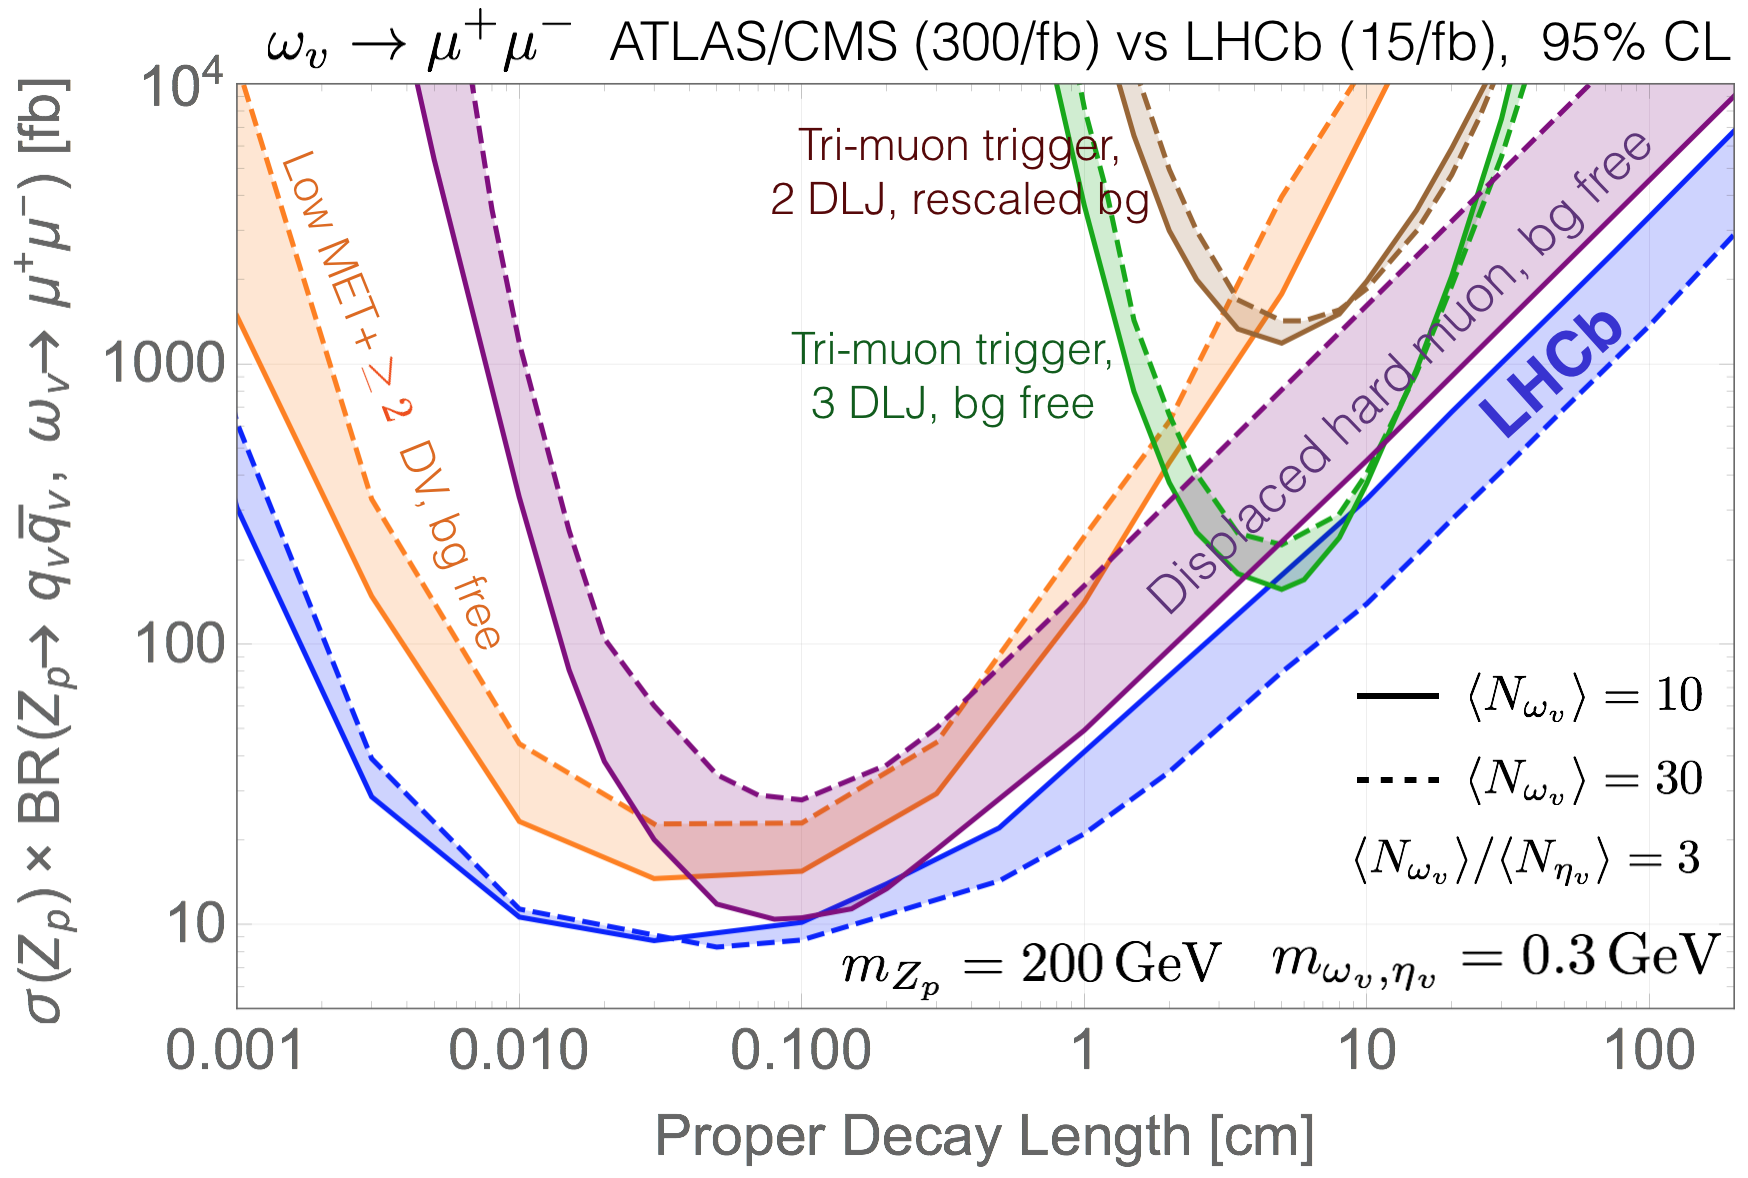
\includegraphics[width=0.8\textwidth]{figures/ulhcb_darkmesons_dileptons.png}}
  \caption{Projected bounds from various ATLAS/CMS searches and the LHCb search for the di-muon~\cite{Pierce:2017taw}.}
  \label{fig:ulhcb_hv_dimuons}
\end{figure}


\subsubsection{Displaced jets}
Signatures with displaced jets are very common in the context of LLP searches. LHCb has already started to explore its potential by using the data collected during Run 1 to search for the following signatures:~a single~\cite{Aaij:2017mic} and a double~\cite{Aaij:2016isa} displaced di-jet, and a single displaced high-multiplicity vertex including a high$-\pt$ muon~\cite{Aaij:2016xmb}. 
Starting with the former signature, already in Run 1 limits have been set on dark-sector pions produced in Higgs decays (analogous to the Higgs production mode and hadronic or semi-leptonic decay modes of the Simplified Models in Chapter \ref{sec:simplifiedmodel}). 

In LHCb Upgrade Ia, the background rejection for displaced-jet searches is expected to improve thanks to the improved VELO resolution. The selection efficiency should also be significantly higher due to the prospects for online displaced vertex identification. 
The main focus of LHCb will be to probe the region at very low lifetime where it has already proven to be the most competitive (see discussion in Section~\ref{sec:experimentcoverage}). The background from QCD and material interactions is the main limiting factor, and the improved vertex resolution of the upgraded VELO together with the lower material budget and the use of a detailed material map are expected to bring large improvements in the upgraded detector.

In some dark-sector models, the number of hadronic displaced vertices can be very large, even in the limited LHCb acceptance (see, for example, Ref.~\cite{Schwaller:2015gea} and the discussion in Chapter \ref{sec:showers}). Typical displaced vertex searches would probably discard these events due to requirements on vertex isolation that are used to remove fake signatures, so a dedicated search strategy is needed. Furthermore, a dedicated software trigger looking for a large number of displaced vertices in the VELO and very soft $\pt$ requirements could in principle be very sensitive to this kind of models, but studies are needed to fully understand its potential and compare LHCb to other experiments.

\subsubsection{Displaced mesons}
SM quark-antiquark pairs from the decay of a low mass particle  often hadronize into SM mesons that subsequently decay with known branching ratios. For example, a dark-sector meson with a displaced decay to $c\bar{c}$ often produces two $D$ mesons which in turn have non-negligible lifetimes. In this scenario, the authors of Ref.~\cite{Pierce:2017taw} have investigated the prospects of using more or less inclusive reconstruction of the two $D$ mesons decays at the upgraded LHCb. A very similar approach could be used to target decays to $b\bar{b}$ that hadronize to $B$ mesons since the latter is very likely to produce $D$ mesons in its decay. Since LHCb is designed to reconstruct heavy-flavor decays, it can be very competitive in this kind of search~\cite{Pierce:2017taw} (see Fig.~\ref{fig:HVlim}). Furthermore, searches for displaced mesons will greatly profit from the software trigger, which is mainly designed to improve the efficiency of similar-looking hadronic decays of heavy flavor mesons.

\begin{figure}[t]
  \centering
  {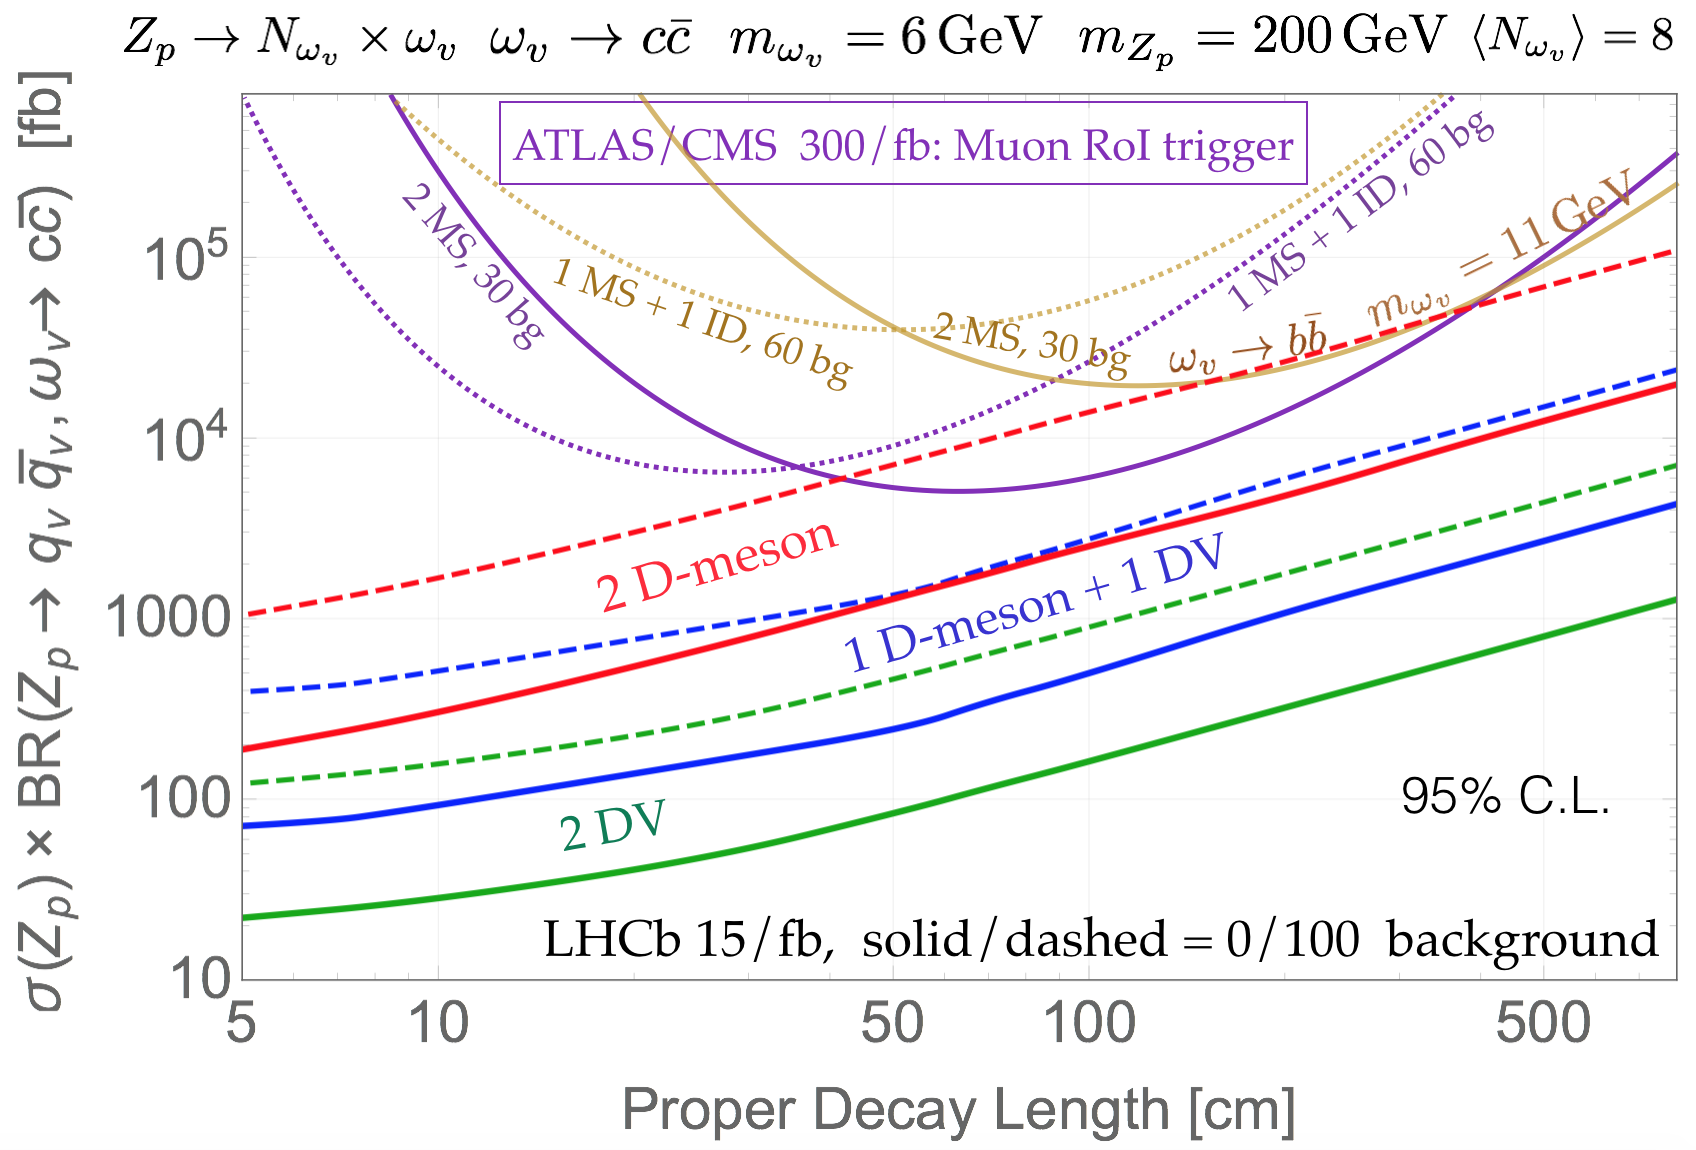
\includegraphics[width=0.8\textwidth]{figures/lhcb_hvlimits2.png}}
  \caption{Projected bounds from various proposed searches for confining hidden valley models exploiting $c\bar{c}$ decays of hidden valley mesons $\omega_v$ (taken from Ref.~\cite{Pierce:2017taw}). The sensitivities with various signatures at LHCb are shown:~two displaced vertices (green), one reconstructed $D$ meson and one DV (blue) and two reconstructed $D$ mesons (red). Searches for this same particular model at ATLAS/CMS are shown not to be competitive (more details can be found in Ref.~\cite{Pierce:2017taw}).}
  \label{fig:HVlim}
\end{figure}

\subsection{After Phase-Ia upgrade: Phase-Ib and Phase-II}
\label{sec:ulhcbphaseii}


After a consolidation phase (Phase Ib) during long shutdown 3 aiming to run in the same conditions as in Phase Ia, the LHCb detector will go through its Phase-II upgrade during long shutdown 4. The Phase-II upgrade is needed to face even more challenging conditions than during previous runs:~for example,ten times higher particle multiplicity, pile-up and radiation damage with respect to Phase-I conditions are expected. The LHCb experiment expects to collect at least 300 \invfb by the end of
Upgrade II~\cite{LHCbUpgradeIIPC}. 

%The LHC will begin operating under high-luminosity conditions
%immediately after LS3, but the LHCb experiment will continue taking data at the same luminosity (thanks to a luminosity scaling at IP8) as that of Run 3. However, minor upgrades to some of the sub-detector systems are foreseen during LS3 (hereafter referred to as ``LHCb consolidation'') \cite{Aaij:2244311}. 
Major improvements to the LHCb detector during Phase Ib and II that are relevant for LLP searches are described in the following, as well as some na\"ive projections of Run-1 results to an an integrated luminosity of 300 \invfb. 

\paragraph{Triggers on downstream tracks}
Most of the LLP searches at the LHCb experiment use the so-called ``long tracks'' to reconstruct the candidates, which are tracks where inputs from both the VELO and the tracking stations are considered. These tracks have an excellent spatial and momentum resolution, and result from an LLP decaying within the VELO region. This is the reason why most the LLP searches done by LHCb correspond to long-lived candidates with displacements typically up to $\mathcal{O}$(10) cm, with the VELO tracking algorithm optimized for displacements of up to 20 cm. However, for long-lived candidates with displacements larger than 20 cm, a different type of track which considers information only from the tracking stations, ``downstream tracks'', has to be used instead of the ``long track'' type. Unfortunately, these tracks have worse vertex and momentum resolution, limiting the capabilities of LHCb for this displacement range. In order to improve the detector sensitivity in the displacement ranges between 20 and 200 cm, a proposal to develop new trigger lines to select ``downstream tracks'' is being studied \cite{Aaij:2244312}. An interesting idea which can help to achieve this tasks and to significantly reduce the CPU computing time, is the implementation of a system of specialized processors used to  rapidly find the downstream tracks through look-up tables, and present these tracks to the software trigger in parallel with all the raw detector information in the event. This system, named ``retina'', is being studied and has its own R\&D programme \cite{Abba:2014iga}. 

\paragraph{Magnet Stations}
Among with the ''long'' and ''downstream'' track types, ``upstream'' tracks are also considered useful for LLP searches. These tracks correspond to soft charged particles bending out of the detector acceptance, produced from LLP candidates which decay within the VELO region. Aside from the installation of a new tracker during LS2, the UT, a proposal to add Magnet Stations (MS) inside the LHCb magnet to improve low momentum resolution is considered \cite{Aaij:2244311}. These MS have been proposed
to be installed for Phase Ib, and are foreseen to highly improve the tracking of low momentum particles produced from certain kind of LLP candidates, such as for example soft pions from ``disappearing'' chargino tracks.

\paragraph{Material interactions}
The presence of a VELO envelope at approximately 5 mm from the beam line in order to separate the VELO and the LHC vacuums, named ``RF-foil'', strongly affects the background composition of LLP searches in the LHCb experiment. Namely, for LLP candidates decaying below 5 mm from the beam line, the main source of background is due to heavy flavour decays; while material interactions with the RF-foil compose the main background contribution for those LLP decaying above 5 mm from the beam line. While the former is purely due to QCD processes and hence not reducible, the latter is kept under control by the use of a very detailed veto map (see Ref.~\cite{Aaij:2017rft}). However, the ideal case would be to completely remove the RF-foil during the Phase-II upgrade \cite{Aaij:2244311}, which would result in a huge reduction of the background component due to material interactions. A removal of the RF-foil in addition with the  improvements foreseen to the Phase-II VELO (probably based on an improved version of the Phase-I VELO), will improve sensitivity to shorter lifetimes, better PV and impact parameter resolution (see Fig.~\ref{fig:veloip_hllhc}), and achieve a real-time alignment. Unfortunately, the removal of the RF-foil is not necessarily seen as a viable option; therefore, improving  the material veto maps as much as possible by accurately modeling the material interactions would be desirable as a more conservative option for the HL-LHC era. 

\begin{figure}[t]
\centerline{
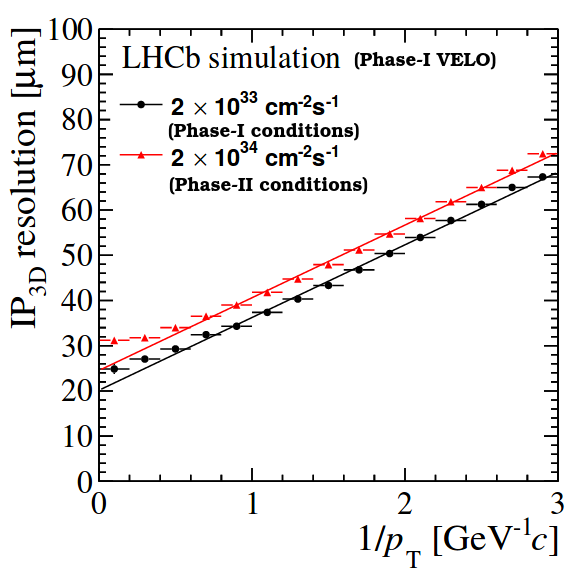
\includegraphics[width=0.48\textwidth]{figures/velo_ph21.png}
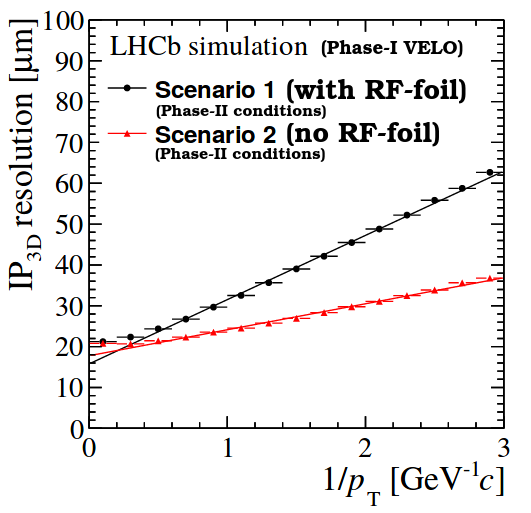
\includegraphics[width=0.48\textwidth]{figures/velo_ph22.png}
}
  \caption{Impact parameter resolution estimations from simulation using the Phase-I VELO model: a comparison if considering Phase-I or Phase-II conditions is shown on the left plot, while the effect of the RF-foil removal under Phase-II conditions is presented on the right plot.}
  \label{fig:veloip_hllhc}
\end{figure}

\paragraph{Na\"ve projections of Run-1 results to the HL-LHC era}

By taking the published Run-1 results from the single displaced dijet search~\cite{Aaij:2017mic} at LHCb, extrapolations to the integrated luminosity foreseen to be recorded by LHCb during Phase-II, 300 \invfb, are presented in Fig.~\ref{fig:dvsearches_hllhc}. These numbers have been obtained by simply scaling signal and background and taking into account the increase in cross section. Very conservative assumptions are considered regarding jet reconstruction efficiencies, trigger efficiencies and material interactions (namely the same numbers as those from Run 1 are taken):~aside from sensible improvements regarding trigger and material interactions as discussed in previous paragraphs, jet reconstruction techniques are foreseen to improve for lower masses due to the implementation of novel tools for disentangling jet substructure. Regarding pile-up effects, considered assumptions are very optimistic (no pile-up effects are considered at all for these extrapolations); however, the impact of pile-up remains to be studied in much detail (especially for those searches involving jets in the final state). 

To mitigate pile-up, there are some ideas under consideration. For example, the removal of neutral tracks (more pile-up dependent than charged tracks) from jet reconstruction; or the use of machine-learning techniques to suppress pile-up contributions. Further studies are needed to arrive at definitive conclusions for the effects of pile-up and its mitigation. 
%% Martino: maybe add somewhere that we are open to new interesting topics? Soft bombs, Rare Z decays to hidden sector, etc.

\begin{figure}[t]
  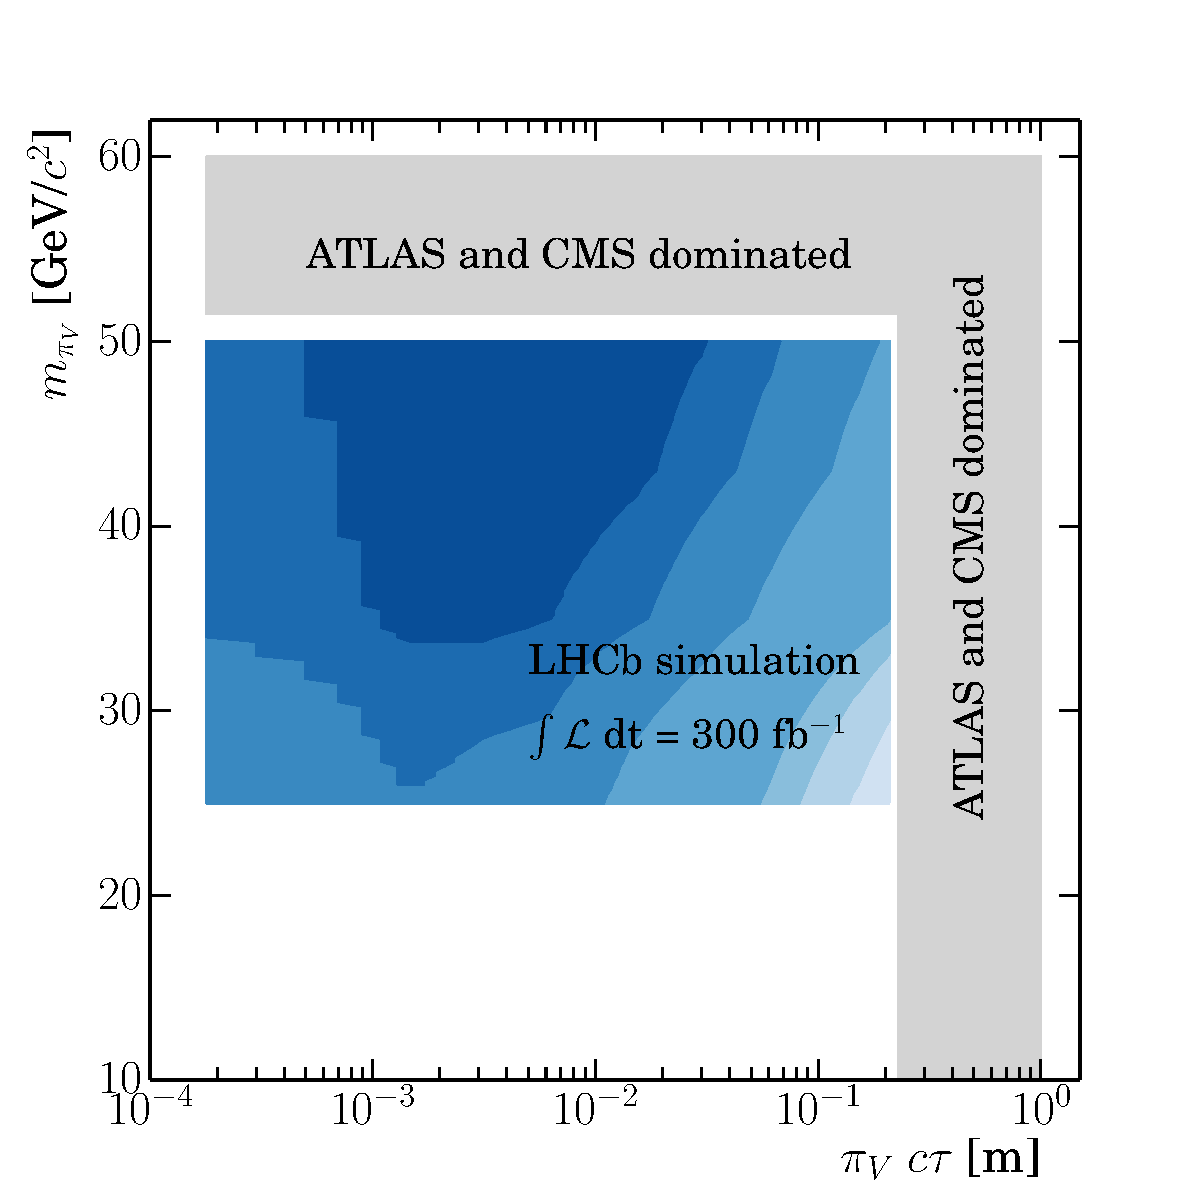
\includegraphics[width=0.65\textwidth]{figures/LLP_compare_PIV_4_HL.pdf}
\begin{minipage}[t]{0.26\textwidth}
  \vspace{-6.cm}
  \hspace{-0.7cm}
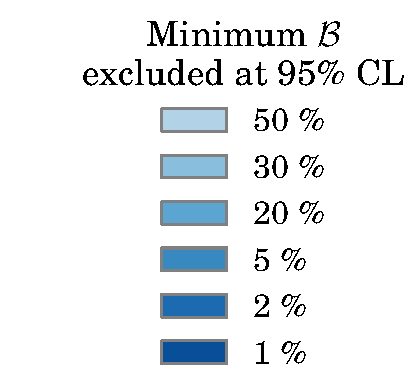
\includegraphics[width=1.2\textwidth]{figures/LLP_compare_legend.pdf}
\end{minipage}
  \caption{Naive sensitivity projections for searches of displaced dijet vertices at LHCb~\cite{Aaij:2017mic} to the expected luminosity to be collected with the Phase-II upgraded detector (300\invfb).}
  \label{fig:dvsearches_hllhc}
\end{figure}

